\documentclass[landscape]{article}
\usepackage[paperwidth=254mm,paperheight=452mm,margin=0mm]{geometry}
\usepackage{tikz}
\usetikzlibrary{calc}
\usepackage{fontspec}
\usepackage{xeCJK}
\usepackage{fancyhdr}
\usepackage{datetime2}
\usepackage{amssymb}
\usepackage{hyperref}

% ハイパーリンク設定
\hypersetup{
    colorlinks=true,
    linkcolor=blue,
    urlcolor=blue,
    pdfborder={0 0 0}
}

% フォント設定
\setmainfont{DejaVu Sans}
\setCJKmainfont{Noto Sans CJK JP}
\setCJKsansfont{Noto Sans CJK JP}

% ヘッダー・フッター設定
\pagestyle{fancy}
\fancyhf{}
\renewcommand{\headrulewidth}{0pt}
\renewcommand{\footrulewidth}{0pt}

% 色設定
\definecolor{lightgray}{RGB}{240,240,240}
\definecolor{medgray}{RGB}{200,200,200}
\definecolor{darkgray}{RGB}{100,100,100}
\definecolor{accent}{RGB}{100,150,200}

\setlength{\parindent}{0pt}
\setlength{\parskip}{0pt}

\begin{document}

% ページ1: Monthly Calendar - January 2025
\hypertarget{monthly-jan}{}
\begin{tikzpicture}[remember picture,overlay]
\node[anchor=north west] at (current page.north west) {
\begin{minipage}[t][452mm][t]{254mm}

% ヘッダー
\begin{tikzpicture}
\fill[accent!30] (0,0) rectangle (254mm,32mm);
\node[anchor=west,font=\fontsize{36}{40}\selectfont\bfseries] at (10mm,16mm) {January 2025};
\node[anchor=east,font=\fontsize{16}{20}\selectfont] at (244mm,16mm) {\hyperlink{weekly-jan-w1}{Weekly View} | \hyperlink{daily-jan-01}{Daily View}};
\end{tikzpicture}

\vspace{5mm}

% カレンダーグリッド
\begin{tikzpicture}[x=1mm,y=1mm]
% 曜日ヘッダー(月曜始まり)
\foreach \x/\day in {0/Mon,1/Tue,2/Wed,3/Thu,4/Fri,5/Sat,6/Sun} {
  \pgfmathsetmacro{\xpos}{10+\x*34.57}
  \pgfmathsetmacro{\xposend}{10+(\x+1)*34.57}
  \pgfmathsetmacro{\xcenter}{\xpos+17.285}
  \fill[lightgray] (\xpos,377) rectangle (\xposend,398);
  \draw[thick] (\xpos,377) rectangle (\xposend,398);
  \node[font=\fontsize{16}{20}\selectfont\bfseries] at (\xcenter,387.5) {\day};
}

% 日付データ(2025年1月 - 水曜始まり)
\def\dates{{0,0,1,2,3,4,5,6,7,8,9,10,11,12,13,14,15,16,17,18,19,20,21,22,23,24,25,26,27,28,29,30,31,0,0}}

% 6週分のグリッド
\foreach \row in {0,1,...,5} {
  \foreach \col in {0,1,...,6} {
    \pgfmathsetmacro{\y}{377-(\row+1)*58.67}
    \pgfmathsetmacro{\yend}{\y+58.67}
    \pgfmathsetmacro{\xpos}{10+\col*34.57}
    \pgfmathsetmacro{\xposend}{10+(\col+1)*34.57}
    \pgfmathsetmacro{\idx}{\row*7+\col}
    \pgfmathsetmacro{\date}{\dates[\idx]}
    
    \draw[thick] (\xpos,\y) rectangle (\xposend,\yend);
    
    % 日付表示
    \ifnum\date>0
      \pgfmathtruncatemacro{\dateint}{\date}
      \node[anchor=north west,font=\fontsize{14}{16}\selectfont] at ({\xpos+2},{\yend-2}) {\hyperlink{daily-jan-\ifnum\dateint<10 0\fi\dateint}{\dateint}};
    \fi
  }
}
\end{tikzpicture}

\end{minipage}
};
\end{tikzpicture}

\newpage

% ページ2: Weekly Schedule - Week 1 (Dec 30 - Jan 5)
\hypertarget{weekly-jan-w1}{}
\begin{tikzpicture}[remember picture,overlay]
\node[anchor=north west] at (current page.north west) {
\begin{minipage}[t][452mm][t]{254mm}

% ヘッダー
\begin{tikzpicture}
\fill[accent!30] (0,0) rectangle (254mm,32mm);
\node[anchor=west,font=\fontsize{36}{40}\selectfont\bfseries] at (10mm,16mm) {Week 1: Dec 30 - Jan 5};
\node[anchor=east,font=\fontsize{16}{20}\selectfont] at (244mm,16mm) {\hyperlink{monthly-jan}{Monthly} | \hyperlink{daily-jan-01}{Daily}};
\end{tikzpicture}

\vspace{5mm}

% 時間軸付き週間表
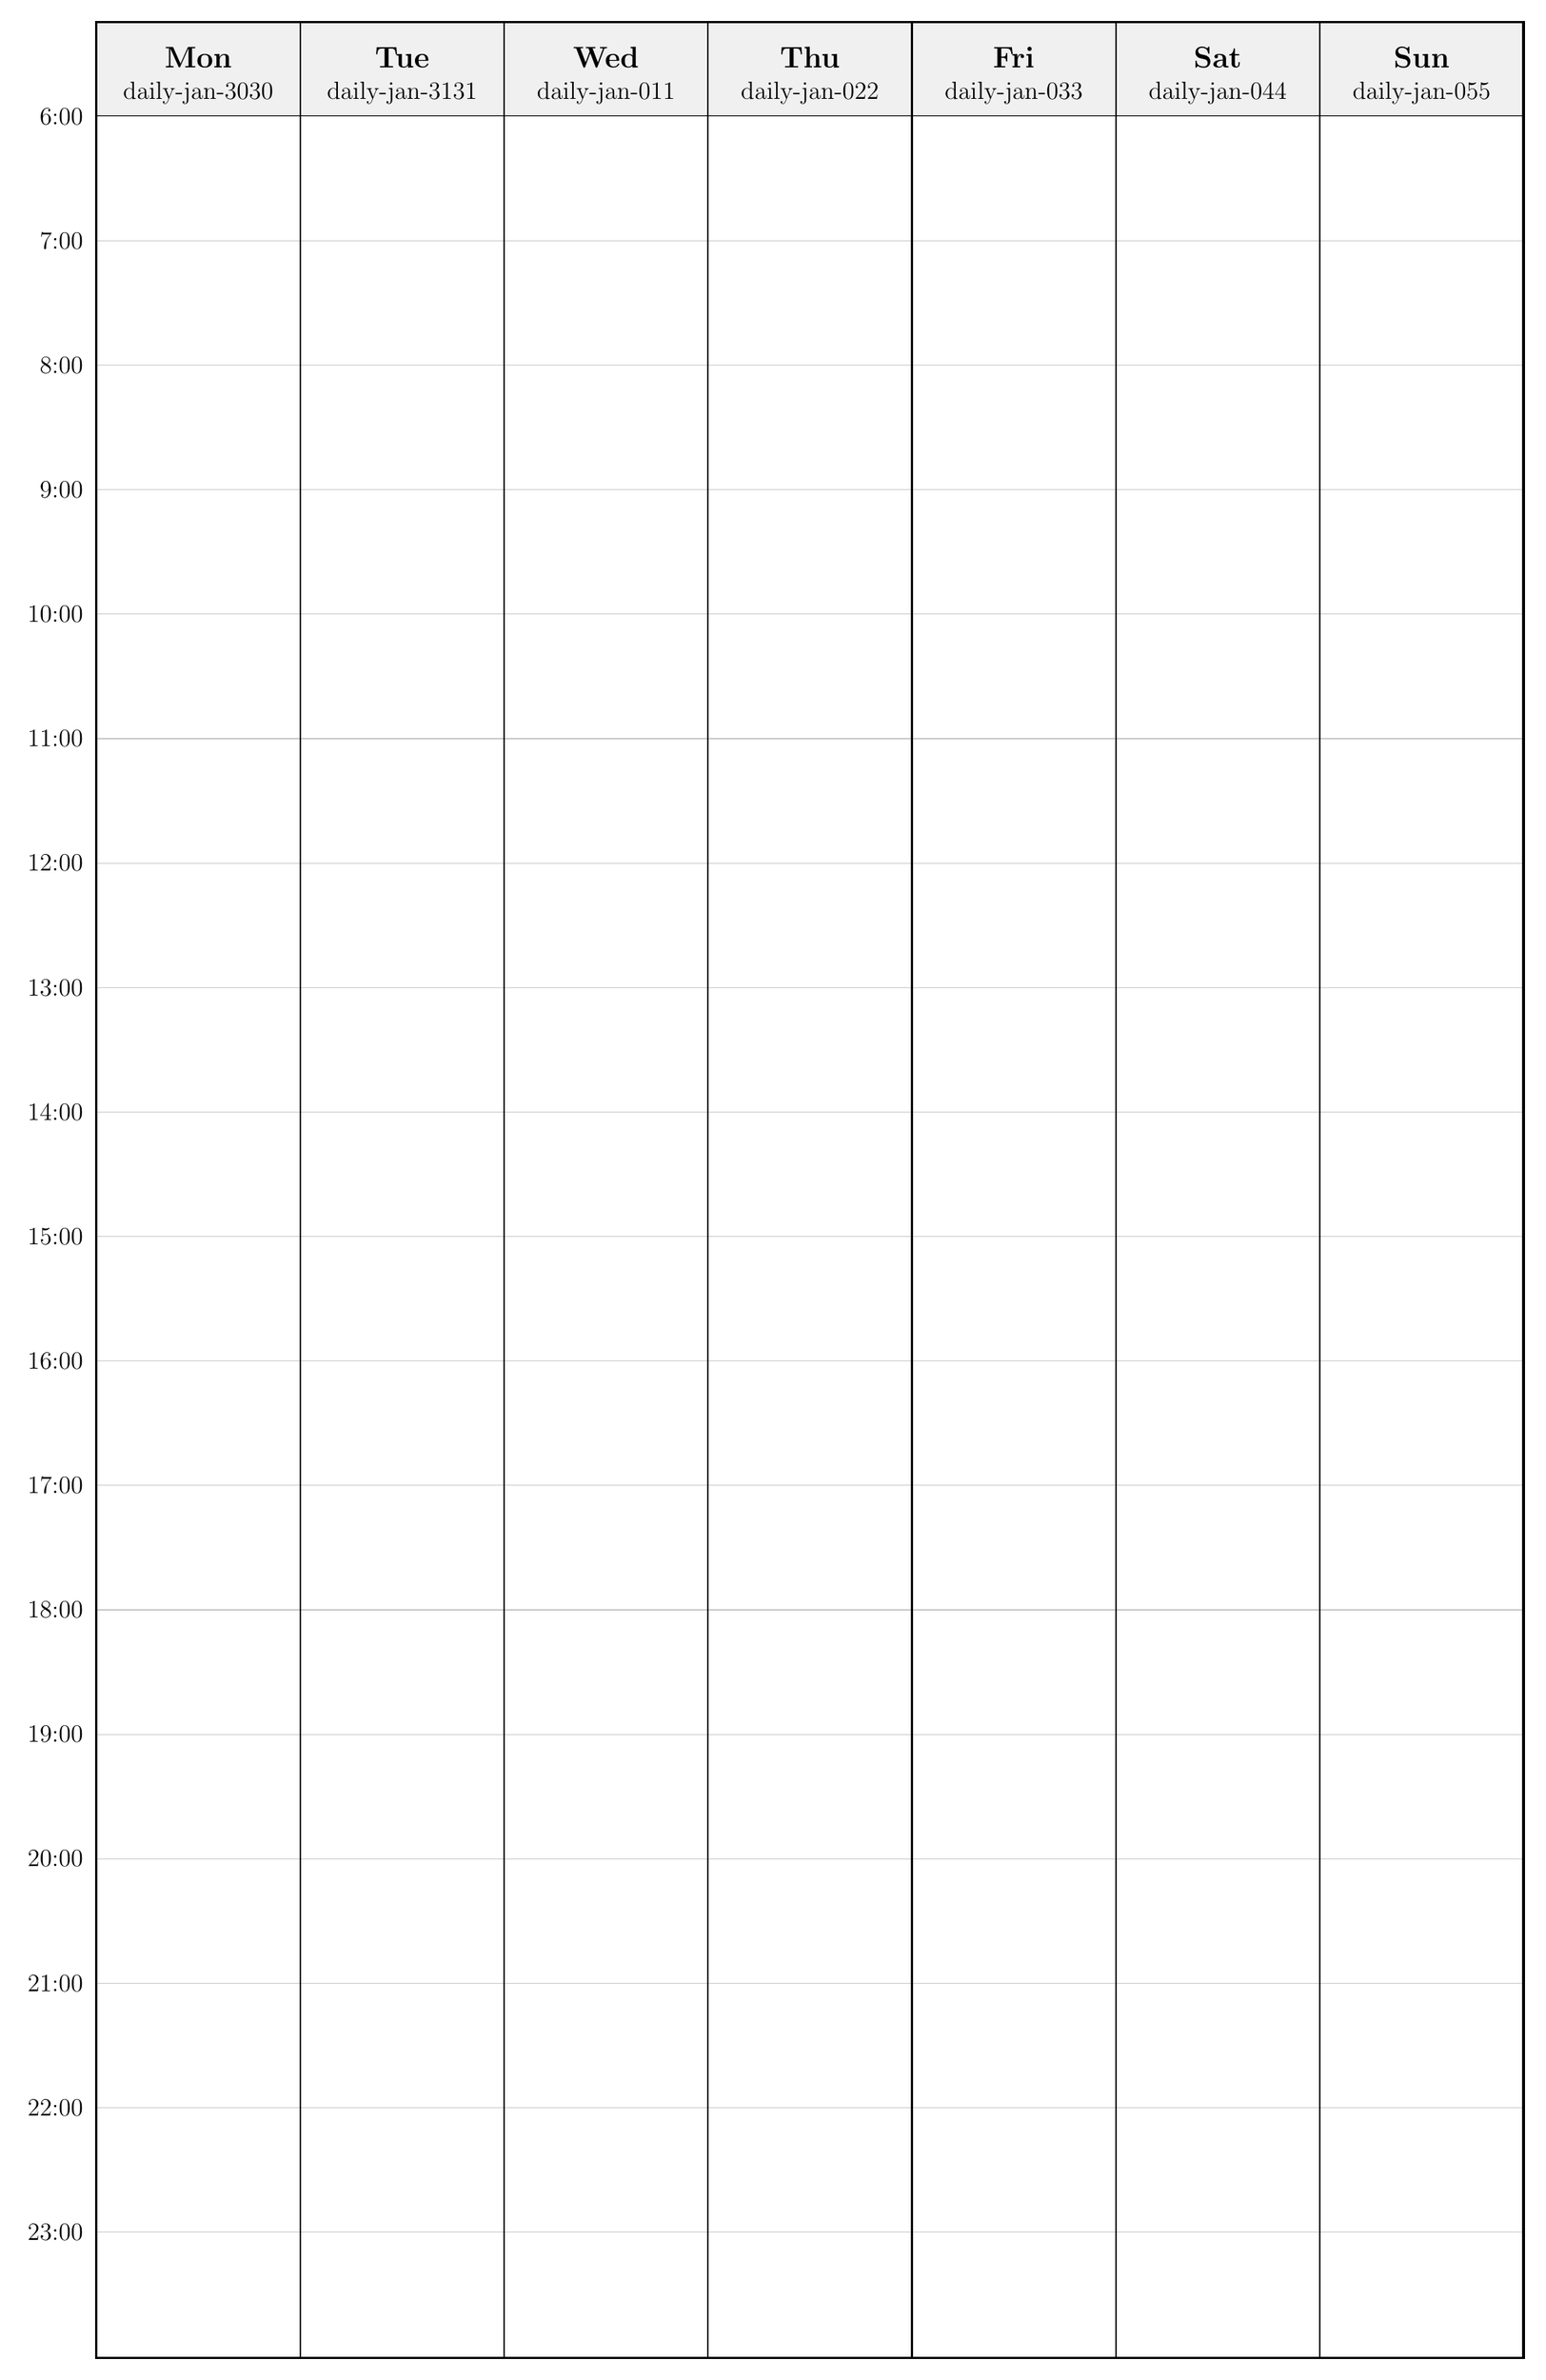
\begin{tikzpicture}[x=1mm,y=1mm]
% 曜日ヘッダー(月曜始まり)
\foreach \x/\day/\date in {0/Mon/30,1/Tue/31,2/Wed/1,3/Thu/2,4/Fri/3,5/Sat/4,6/Sun/5} {
  \pgfmathsetmacro{\xpos}{10+\x*34.57}
  \pgfmathsetmacro{\xposend}{10+(\x+1)*34.57}
  \fill[lightgray] (\xpos,380) rectangle (\xposend,396);
  \draw[thick] (\xpos,380) rectangle (\xposend,396);
  \pgfmathsetmacro{\xcenter}{\xpos+17.285}
  \node[font=\fontsize{14}{18}\selectfont\bfseries] at (\xcenter,390) {\day};
  \node[font=\fontsize{12}{14}\selectfont] at (\xcenter,384) {\hyperlink{daily-jan-\ifnum\date<10 0\fi\date}{\date}};
}

% 時間軸と罫線
\foreach \h in {6,7,...,23} {
  \pgfmathsetmacro{\y}{380-(\h-6)*21.1}
  \draw[medgray] (10,\y) -- (252,\y);
  \node[anchor=east,font=\fontsize{12}{14}\selectfont] at (9,\y) {\h:00};
}

% 縦線(曜日の区切り)
\foreach \x in {0,1,...,7} {
  \pgfmathsetmacro{\xpos}{10+\x*34.57}
  \draw[thick] (\xpos,0) -- (\xpos,396);
}

% 外枠
\draw[very thick] (10,0) rectangle (252,396);
\end{tikzpicture}

\end{minipage}
};
\end{tikzpicture}

\newpage

% ページ3: Daily Planner - January 1, 2025 (Wednesday)
\hypertarget{daily-jan-01}{}
\begin{tikzpicture}[remember picture,overlay]
\node[anchor=north west] at (current page.north west) {
\begin{minipage}[t][452mm][t]{254mm}

% ヘッダー
\begin{tikzpicture}
\fill[accent!30] (0,0) rectangle (254mm,32mm);
\node[anchor=west,font=\fontsize{36}{40}\selectfont\bfseries] at (10mm,16mm) {Wednesday, January 1};
\node[anchor=east,font=\fontsize{16}{20}\selectfont] at (244mm,16mm) {\hyperlink{monthly-jan}{Monthly} | \hyperlink{weekly-jan-w1}{Weekly}};
\end{tikzpicture}

\vspace{5mm}

% 左側:時間割
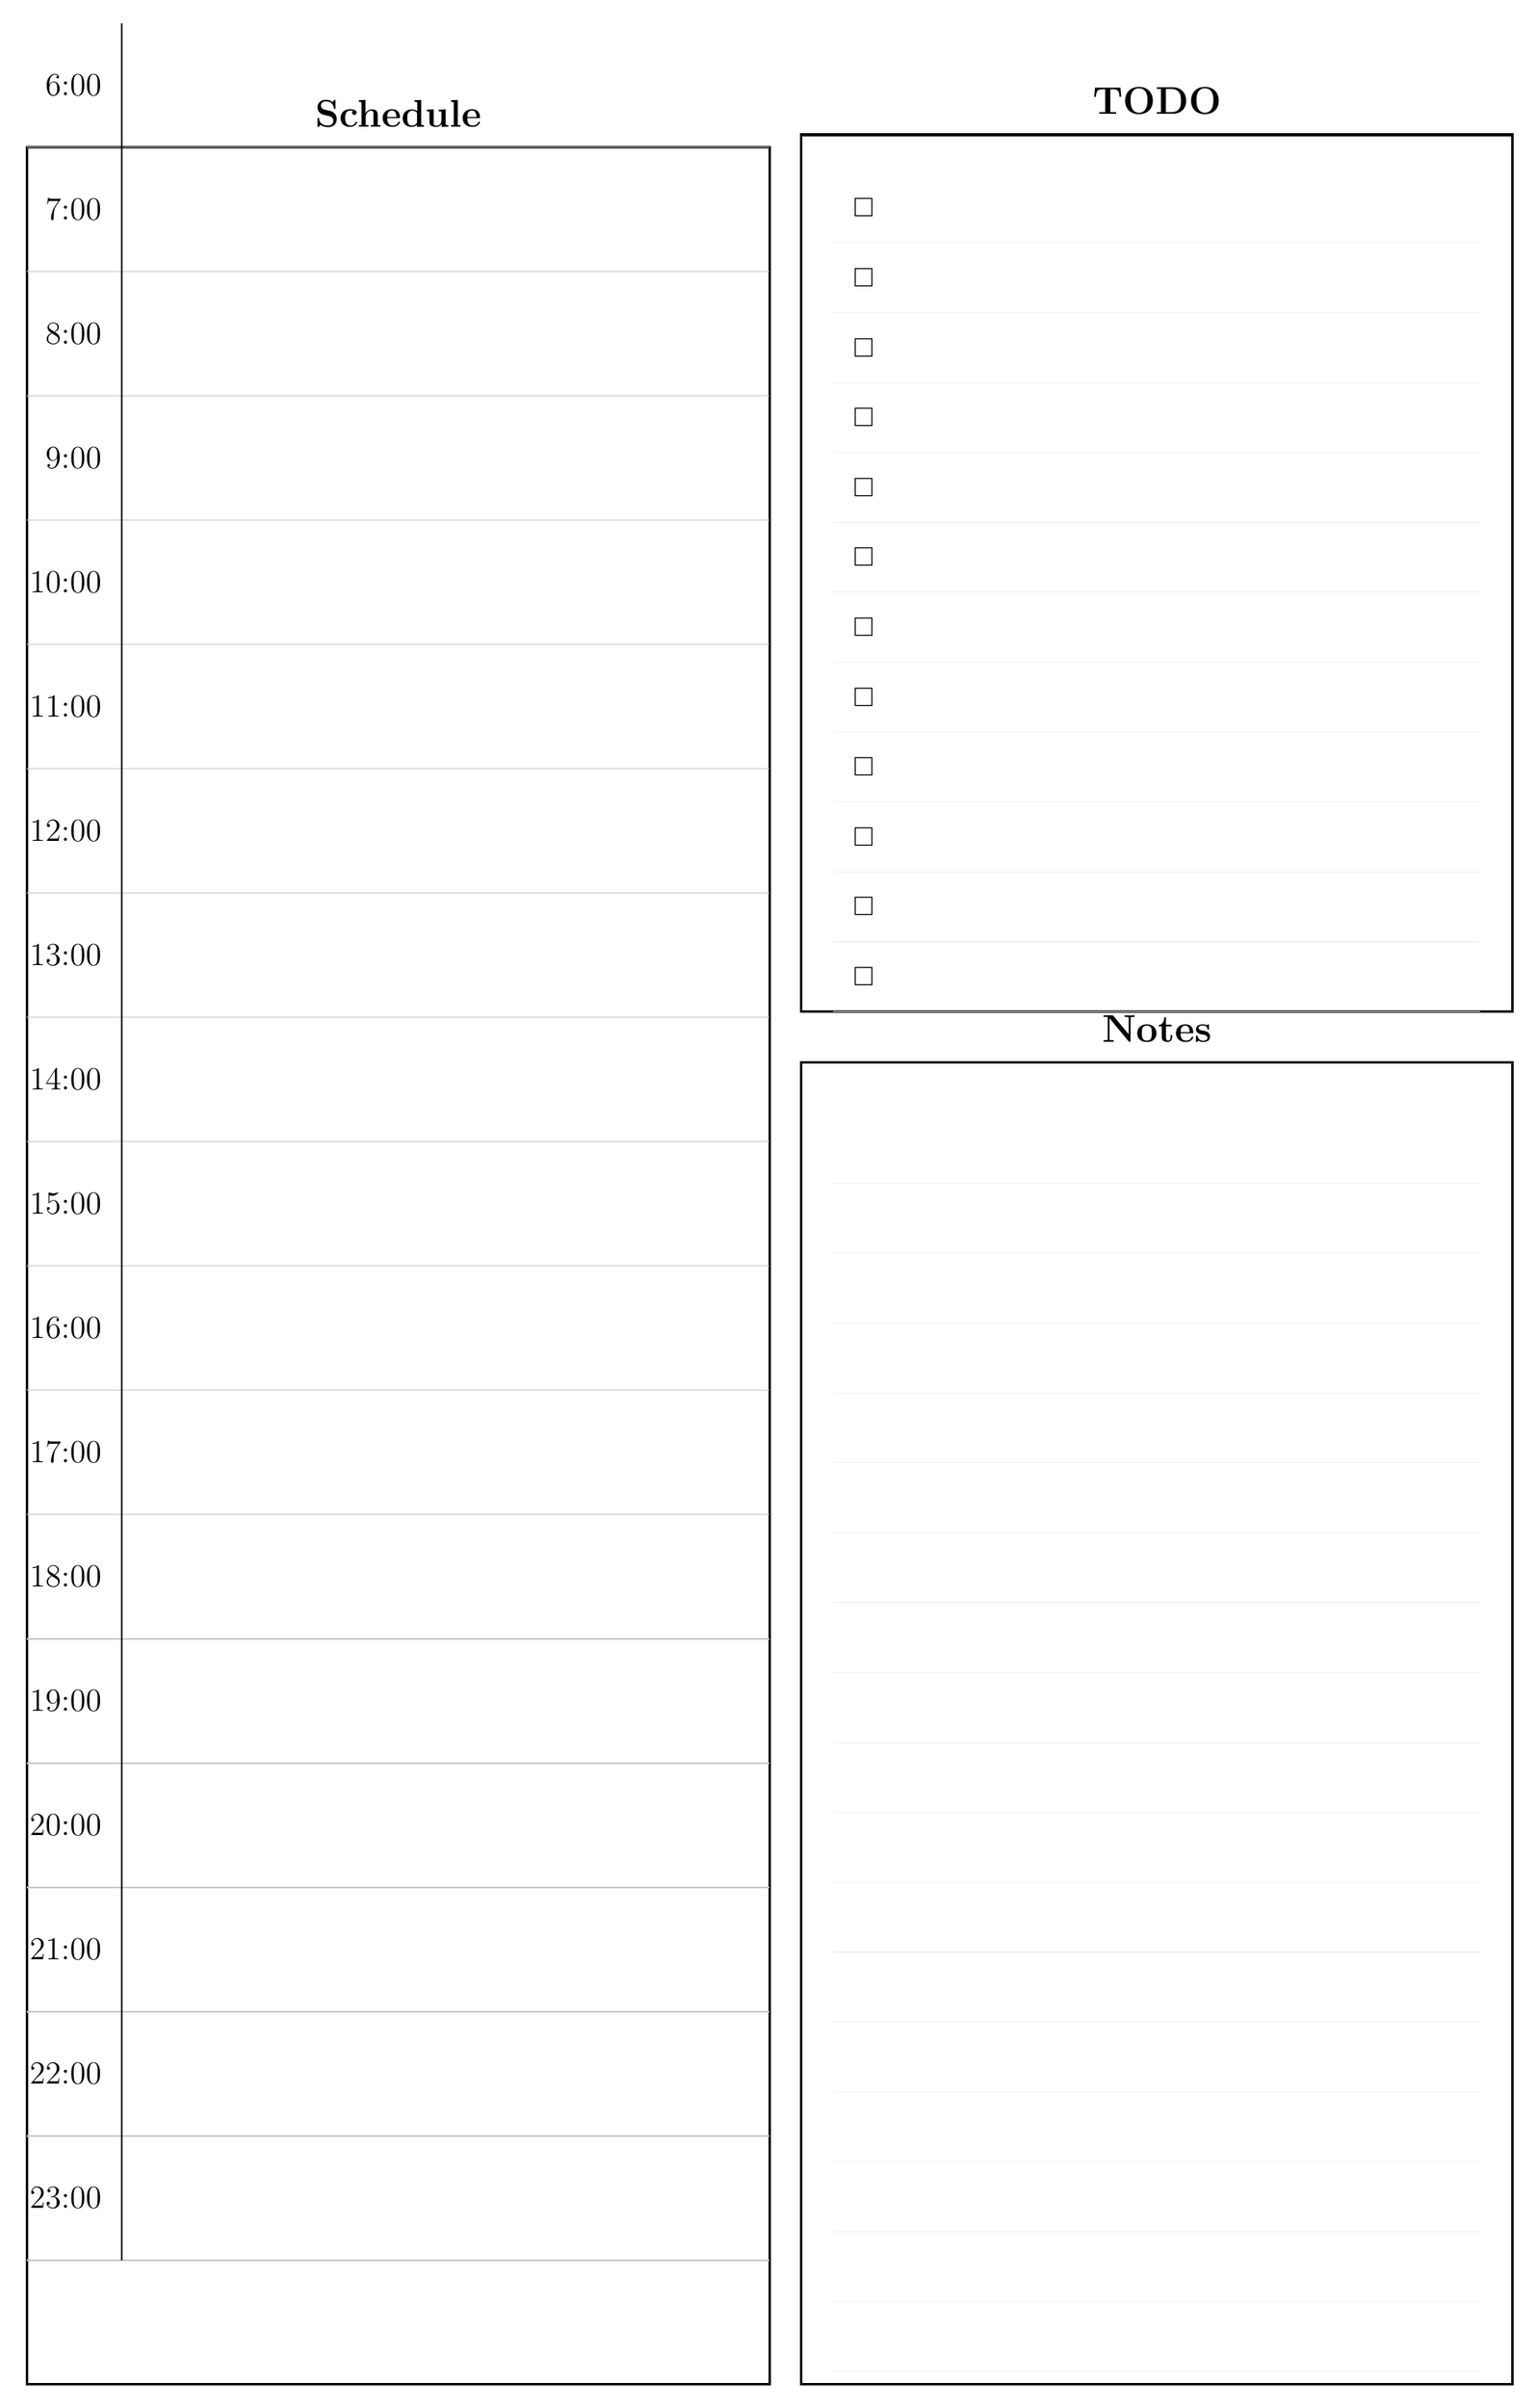
\begin{tikzpicture}[x=1mm,y=1mm]
% 時間軸
\draw[very thick] (10,20) rectangle (127,372);
\node[anchor=south,font=\fontsize{16}{20}\selectfont\bfseries] at (68.5,374) {Schedule};

\foreach \h in {6,7,...,23} {
  \pgfmathsetmacro{\y}{372-(\h-6)*19.56}
  \pgfmathsetmacro{\yend}{\y+19.56}
  \pgfmathsetmacro{\ycenter}{\y+9.78}
  \draw[medgray] (10,\y) -- (127,\y);
  \node[anchor=east,font=\fontsize{14}{16}\selectfont] at (23,\ycenter) {\h:00};
  \draw[thick] (25,\y) -- (25,\yend);
}

% 右側:TODO & Notes
\draw[very thick] (132,236) rectangle (244,374);
\node[anchor=south,font=\fontsize{16}{20}\selectfont\bfseries] at (188,376) {TODO};

\foreach \i in {1,2,...,12} {
  \pgfmathsetmacro{\y}{368-\i*11}
  \pgfmathsetmacro{\ycenter}{\y+5.5}
  \draw[lightgray] (137,\y) -- (239,\y);
  \node[anchor=west,font=\fontsize{12}{14}\selectfont] at (139,\ycenter) {$\square$};
}

% Notesエリア
\draw[very thick] (132,20) rectangle (244,228);
\node[anchor=south,font=\fontsize{16}{20}\selectfont\bfseries] at (188,230) {Notes};

\foreach \i in {1,2,...,18} {
  \pgfmathsetmacro{\y}{220-\i*11}
  \draw[lightgray] (137,\y) -- (239,\y);
}
\end{tikzpicture}

\end{minipage}
};
\end{tikzpicture}

\newpage

% ページ4: Daily Planner - January 2, 2025 (Thursday)
\hypertarget{daily-jan-02}{}
\begin{tikzpicture}[remember picture,overlay]
\node[anchor=north west] at (current page.north west) {
\begin{minipage}[t][452mm][t]{254mm}

% ヘッダー
\begin{tikzpicture}
\fill[accent!30] (0,0) rectangle (254mm,32mm);
\node[anchor=west,font=\fontsize{36}{40}\selectfont\bfseries] at (10mm,16mm) {Thursday, January 2};
\node[anchor=east,font=\fontsize{16}{20}\selectfont] at (244mm,16mm) {\hyperlink{monthly-jan}{Monthly} | \hyperlink{weekly-jan-w1}{Weekly}};
\end{tikzpicture}

\vspace{5mm}

% 左側:時間割
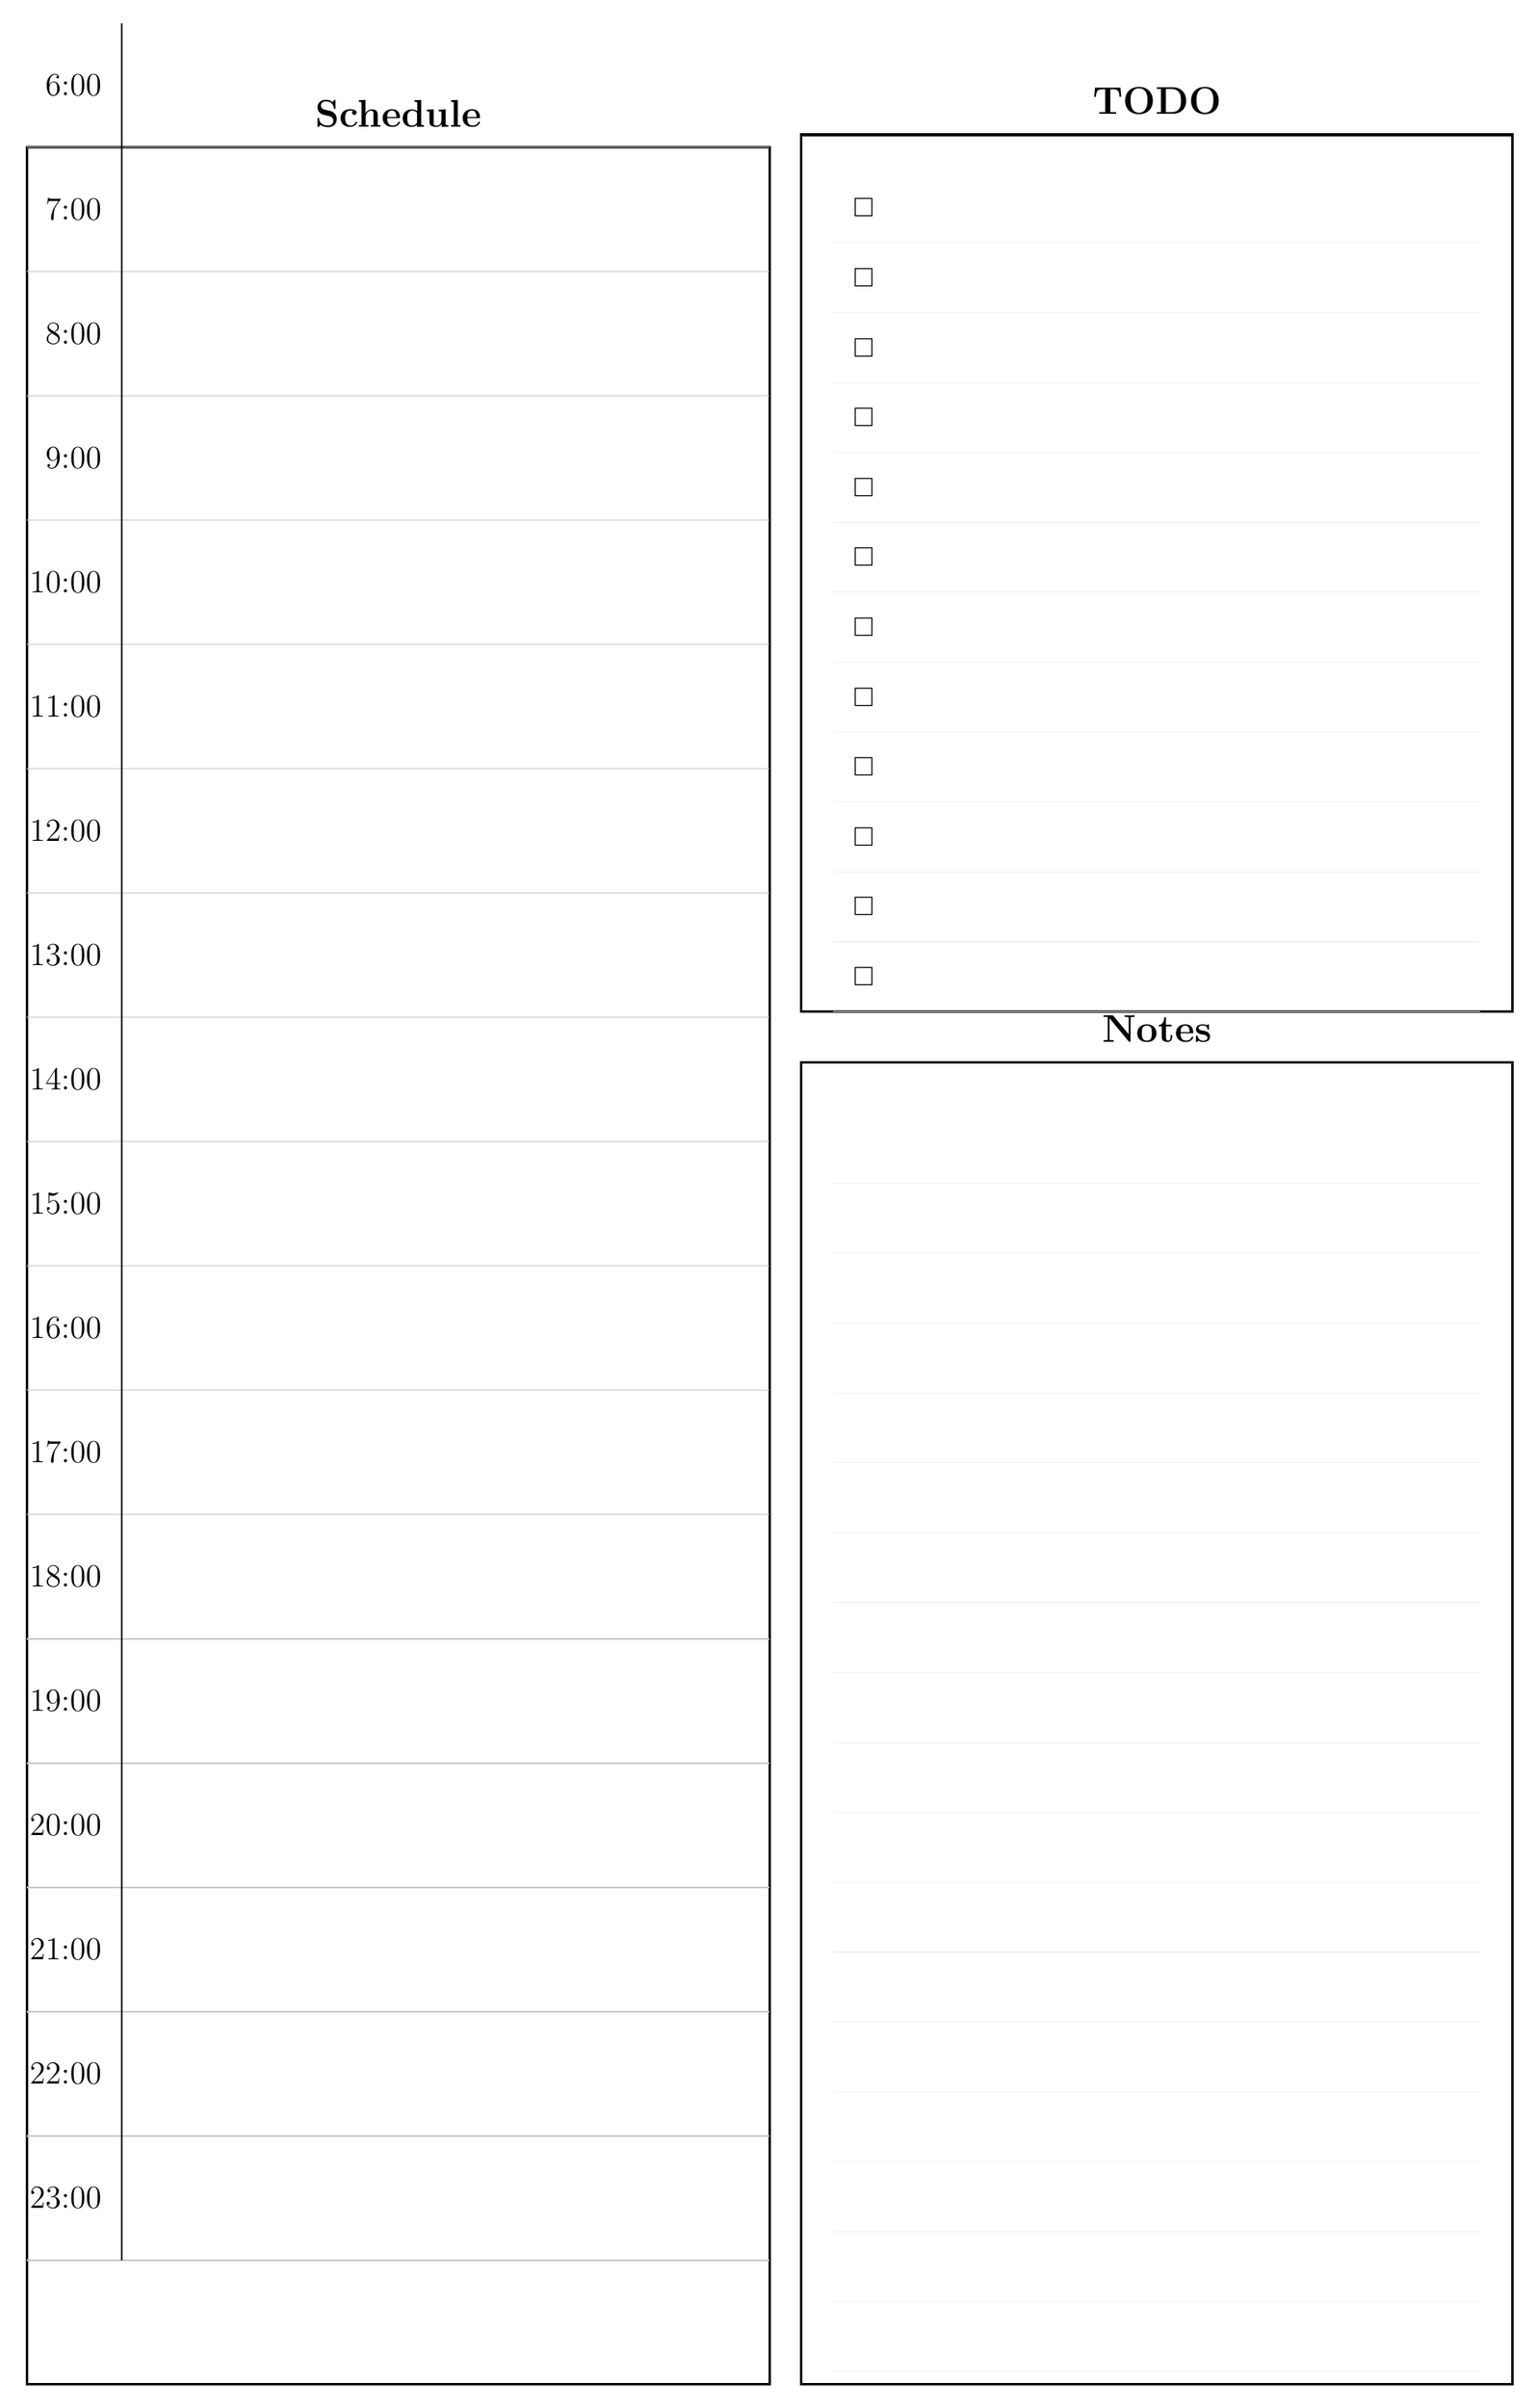
\begin{tikzpicture}[x=1mm,y=1mm]
\draw[very thick] (10,20) rectangle (127,372);
\node[anchor=south,font=\fontsize{16}{20}\selectfont\bfseries] at (68.5,374) {Schedule};

\foreach \h in {6,7,...,23} {
  \pgfmathsetmacro{\y}{372-(\h-6)*19.56}
  \pgfmathsetmacro{\yend}{\y+19.56}
  \pgfmathsetmacro{\ycenter}{\y+9.78}
  \draw[medgray] (10,\y) -- (127,\y);
  \node[anchor=east,font=\fontsize{14}{16}\selectfont] at (23,\ycenter) {\h:00};
  \draw[thick] (25,\y) -- (25,\yend);
}

\draw[very thick] (132,236) rectangle (244,374);
\node[anchor=south,font=\fontsize{16}{20}\selectfont\bfseries] at (188,376) {TODO};

\foreach \i in {1,2,...,12} {
  \pgfmathsetmacro{\y}{368-\i*11}
  \pgfmathsetmacro{\ycenter}{\y+5.5}
  \draw[lightgray] (137,\y) -- (239,\y);
  \node[anchor=west,font=\fontsize{12}{14}\selectfont] at (139,\ycenter) {$\square$};
}

\draw[very thick] (132,20) rectangle (244,228);
\node[anchor=south,font=\fontsize{16}{20}\selectfont\bfseries] at (188,230) {Notes};

\foreach \i in {1,2,...,18} {
  \pgfmathsetmacro{\y}{220-\i*11}
  \draw[lightgray] (137,\y) -- (239,\y);
}
\end{tikzpicture}

\end{minipage}
};
\end{tikzpicture}

\end{document}